\documentclass[a4paper,11pt]{article}
%\documentclass[a4paper,11pt,twocolumn]{article}%twocolumn layout; not sure if this works correctly. Feel free to experiment.
\usepackage[pdftex]{color,graphicx}
\usepackage[T1]{fontenc}
\usepackage{pxfonts}
\usepackage{subfigure}
\usepackage{xcolor}
\usepackage[table]{xcolor}
\usepackage{tabularx}
\usepackage{algorithm}
\usepackage[noend]{algpseudocode}
\usepackage{caption}
\usepackage{subcaption}
%color links to figs, etc.
%\usepackage[pdftex,colorlinks,urlcolor=blue,breaklinks]{hyperref}
\usepackage[pdftex,colorlinks]{hyperref}
\hypersetup{colorlinks,%
		    citecolor=black,%
		    filecolor=black,%
		    linkcolor=black,%
		    urlcolor=black,%
		    breaklinks=true,%
		    pdftex}
		    
%easily manipulate margins
\usepackage{geometry}
\makeatletter
\if@twocolumn%
	\geometry{twoside,
		paperwidth=210mm,
  		paperheight=297mm,
  		textheight=682pt,
  		textwidth=516pt,
  		centering,
  		headheight=50pt,
  		headsep=12pt,
  		footskip=18pt,
  		footnotesep=24pt plus 2pt minus 12pt,
 		columnsep=14pt}	
\else%if using twocolumns, I still need to modify the textwidth to accomodate the watermark
	\geometry{twoside,
		  paperwidth=210mm,
		  paperheight=297mm,
		  textheight=750pt,
		  textwidth=500pt,
		  centering,
		  headheight=50pt,
		  headsep=12pt,
		  footskip=18pt,
		  footnotesep=24pt plus 2pt minus 12pt}
\fi%

%change the font
\usepackage{charter}

%CC logos to add in the footer
% \usepackage{ccicons}

%easily manipulate color
\usepackage{color}

\usepackage[utf8]{inputenc} % allow utf-8 input
\usepackage[T1]{fontenc}    % use 8-bit T1 fonts
\usepackage{hyperref}       % hyperlinks
\usepackage{url}            % simple URL typesetting
\usepackage{booktabs}       % professional-quality tables
\usepackage{amsfonts}       % blackboard math symbols
\usepackage{nicefrac}       % compact symbols for 1/2, etc.
\usepackage{microtype}      % microtypography
\usepackage{xcolor}         % colors
\usepackage{amsmath}
\usepackage{algorithmicx}
\usepackage{algorithm, algpseudocode}
\usepackage{graphicx}
\usepackage{adjustbox}
\usepackage{mathrsfs}
\usepackage{amssymb}

%nicely print bioRxiv
\newcommand{\biorxiv}{\emph{bio{\color{red}R}$\chi$iv}}

%add biorxiv type of article using the package background
\usepackage{tikz}
\usepackage[firstpage=True]{background}


\newcommand{\newresults}{
\makeatletter
\if@twocolumn%
	\backgroundsetup{
		position={0.572\paperwidth,-0.025\paperheight} ,
		angle=270,
		color=black,
		opacity=0.60,
		scale=1.5,
		contents={\tikz\node[text=black,fill=gray!40,align=left, minimum width=2.3cm,minimum height=0.6cm,inner sep=0]{New Results};}}
\else
	\backgroundsetup{
		position={0.338\paperwidth,-0.06\paperheight} ,
		angle=270,
		color=black,
		opacity=0.60,
		scale=2.5,
		contents={\tikz\node[text=black,fill=gray!40,align=left, minimum width=2.3cm,minimum height=0.6cm,inner sep=0]{New Results};}}
\fi%
}

\newcommand{\confirmatoryresults}{
\makeatletter
\if@twocolumn%
\backgroundsetup{
	position={0.572\paperwidth,-0.03\paperheight} ,
	angle=270,
	color=black,
	opacity=0.60,
	scale=1.5,
	contents={\tikz\node[text=black,fill=gray!40,align=left, minimum width=3.9cm,minimum height=0.6cm,inner sep=0]{Confirmatory Results};}}
\else
	\backgroundsetup{
	position={0.338\paperwidth,-0.07\paperheight} ,
	angle=270,
	color=black,
	opacity=0.60,
	scale=2.5,
	contents={\tikz\node[text=black,fill=gray!40,align=left, minimum width=3.9cm,minimum height=0.6cm,inner sep=0]{Confirmatory Results};}}
\fi%
}

\newcommand{\contradictoryresults}{
\makeatletter
\if@twocolumn%
	\backgroundsetup{
	position={0.572\paperwidth,-0.03\paperheight} ,
	angle=270,
	color=black,
	opacity=0.0,
	scale=1.5,
	contents={\tikz\node[text=black,fill=gray!40,align=left, minimum width=4.0cm,minimum height=0.6cm,inner sep=0]{};}}
\else
	\backgroundsetup{
	position={0.338\paperwidth,-0.07\paperheight} ,
	angle=270,
	color=black,
	opacity=0.0,
	scale=2.5,
	contents={\tikz\node[text=black,fill=gray!40,align=left, minimum width=4.0cm,minimum height=0.6cm,inner sep=0]{};}}
\fi%
}

%enhanced floats
\usepackage{float}

%rotate floats if necessary
\usepackage{rotating}

%nicer, clever tables, uncomment if necessary
\usepackage{supertabular}

%tables with notes, etc., uncomment if necessary
%\usepackage{threeparttable}

%improved captions, uncomment if necessary
\usepackage{caption}

%add an author block
\usepackage{authblk}
%redefine authorblock font size and affiliation font size
\renewcommand\Authfont{\small}
\renewcommand\Affilfont{\scriptsize}

%add nice headers
\usepackage{fancyhdr}
\pagestyle{fancy}
\renewcommand{\headrulewidth}{0pt}
\lhead{{\footnotesize }}
\chead{}
\rhead{{\footnotesize }}
\lfoot{\ccbynd}
\cfoot{\thepage}
% \rfoot{\biorxiv}


\usepackage{draftwatermark}
\makeatletter
\if@twocolumn
	\SetWatermarkText{}
	\SetWatermarkScale{0.20}
	\SetWatermarkAngle{270}
	%note: I defined this commands in the draftwatermark.sty file. For some reason they are in teh manual but not in the sty file...
	\SetWatermarkHorCenter{0.97\paperwidth}
	\SetWatermarkVerCenter{-.88\paperheight}
\else
	\SetWatermarkText{}
	\SetWatermarkScale{0.25}
	\SetWatermarkAngle{270}
	%note: I defined this commands in the draftwatermark.sty file. For some reason they are in teh manual but not in the sty file...
	\SetWatermarkHorCenter{0.95\paperwidth}
	\SetWatermarkVerCenter{-.82\paperheight}
\fi

%uncomment the type of bioRxiv preprint below to added to the first page
%\newresults{}
%\confirmatoryresults{}
\contradictoryresults{}

%flushleft the title, authorblock and Abstract
%modified from http://tex.stackexchange.com/questions/85343/left-align-abstract-title-and-authors
\makeatletter
\renewcommand{\maketitle}{\bgroup\setlength{\parindent}{0pt}
\begin{flushleft}
  \thispagestyle{plain}
  \textbf{\@title}

  \@author
\end{flushleft}\egroup
}
\makeatother

%redefine the abstract
\renewenvironment{abstract}
 {\small
  \begin{flushleft}
  \textbf{\abstractname}\vspace{-0.40em}\vspace{0pt}
  \end{flushleft}
  \list{}{
    \setlength{\leftmargin}{0cm}%
    \setlength{\rightmargin}{\leftmargin}%
  }%
  \item\relax}
 {\endlist}

\hyphenation{}

\renewcommand*{\thefootnote}{\fnsymbol{footnote}}

%if to do notes need to be added: need to configure this!
\usepackage[colorinlistoftodos]{todonotes}

%feel free to change the reference style to suit your needs
\usepackage[firstinits=true, backref=false, maxcitenames=1,  hyperref=auto, style=authoryear, defernumbers=true, backend=bibtex]{biblatex}[2010/11-19]
\setlength\bibitemsep{1.2\baselineskip}

%change the name of this file to point to your bib file.
\bibliography{./Bibliography/Literature}

\newcommand{\yz}[1]{{\color{blue}[Yizi: #1]}}

\definecolor{dodgerblue}{rgb}{0.12, 0.56, 1.0}
\definecolor{lightseagreen}{rgb}{0.13, 0.7, 0.67}
\definecolor{mediumorchid}{rgb}{0.73, 0.33, 0.83}
\definecolor{electriclavender}{rgb}{0.96, 0.73, 1.0}
\definecolor{royalazure}{rgb}{0.0, 0.22, 0.66}
\definecolor{cadetgray}{rgb}{0.57, 0.64, 0.69}
\definecolor{applegreen}{rgb}{0.55, 0.71, 0.0}
\definecolor{darkpastelpurple}{rgb}{0.59, 0.44, 0.84}
\definecolor{purpleheart}{rgb}{0.41, 0.21, 0.61}



\begin{document}

%always keep the \newline command at the end of the title to add space between the title and the authors
\title{\Large Computer Vision CS-GY 6643 - Homework 1
\newline}
\author{Anushk Pandey, ap7151@nyu.edu}



\date{}

\maketitle
%\tableofcontents


\section{Connectivity: Connected Component Labeling}
\textbf{Jordan's Theorem:} Every simple closed curve in a plane
separates the plane into two connected nonempty sets: an interior region
and an exterior region.

% insert image from question
\subsection{Applying d4 connectivity}

d4 connectivity is defined as the connectivity of a pixel to the neighbors on its vertical and horizontal axes (Akin to a rook in chess). \newline
\begin{figure}[h]
    \centering
    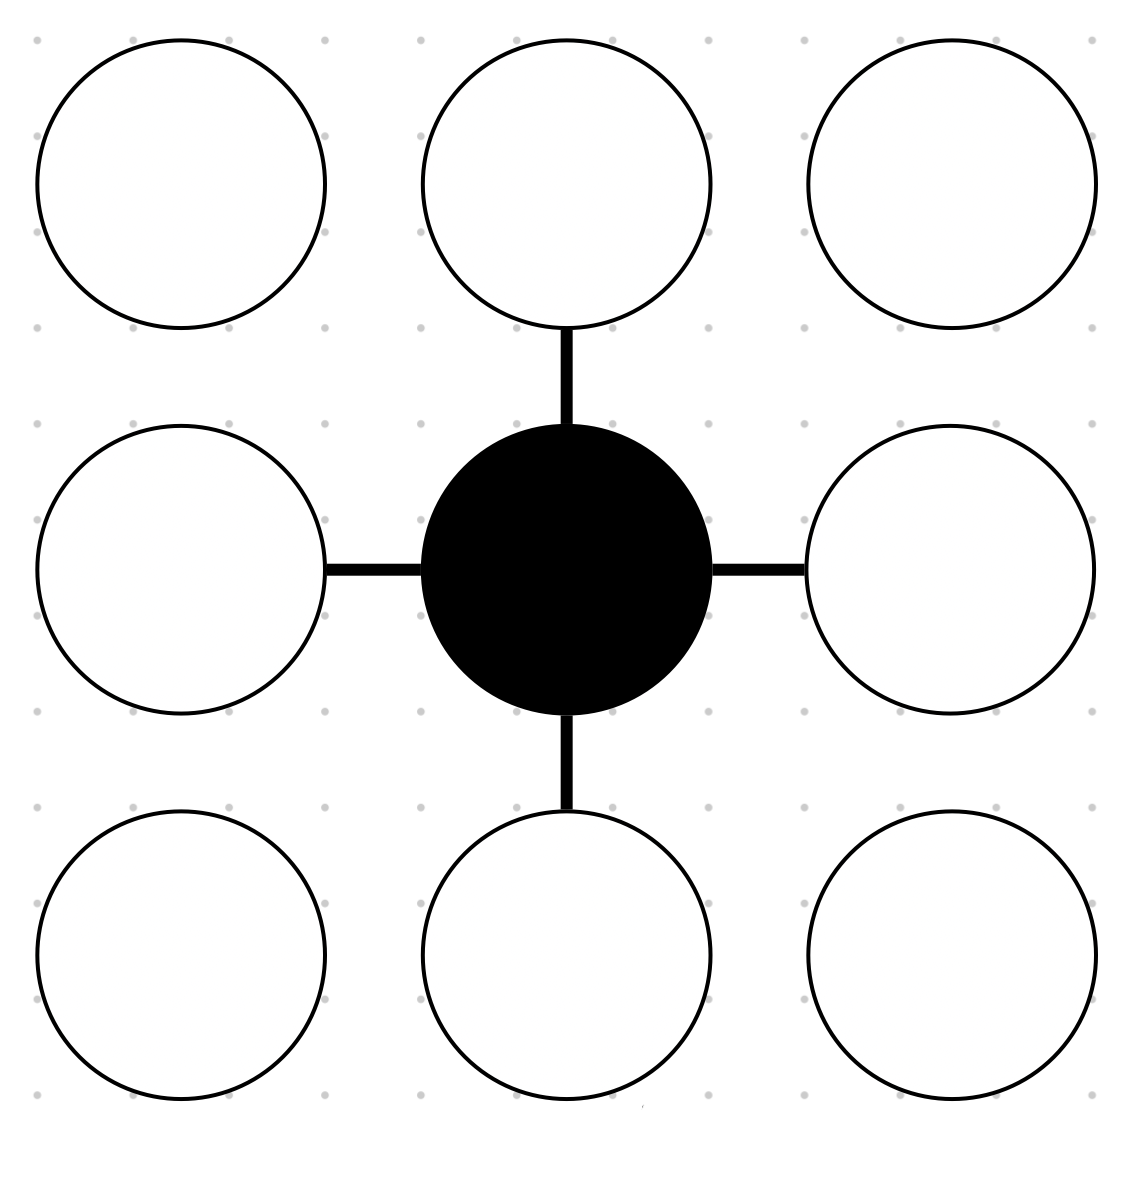
\includegraphics[width=0.3\linewidth]{figs/d4_connectivity.png}
    \caption{An example of $d_4$ connectivity}
\end{figure}
\newline
On computing the d4 connectivity of the given image, we get the following regions:
\begin{figure}[h]
    \centering
    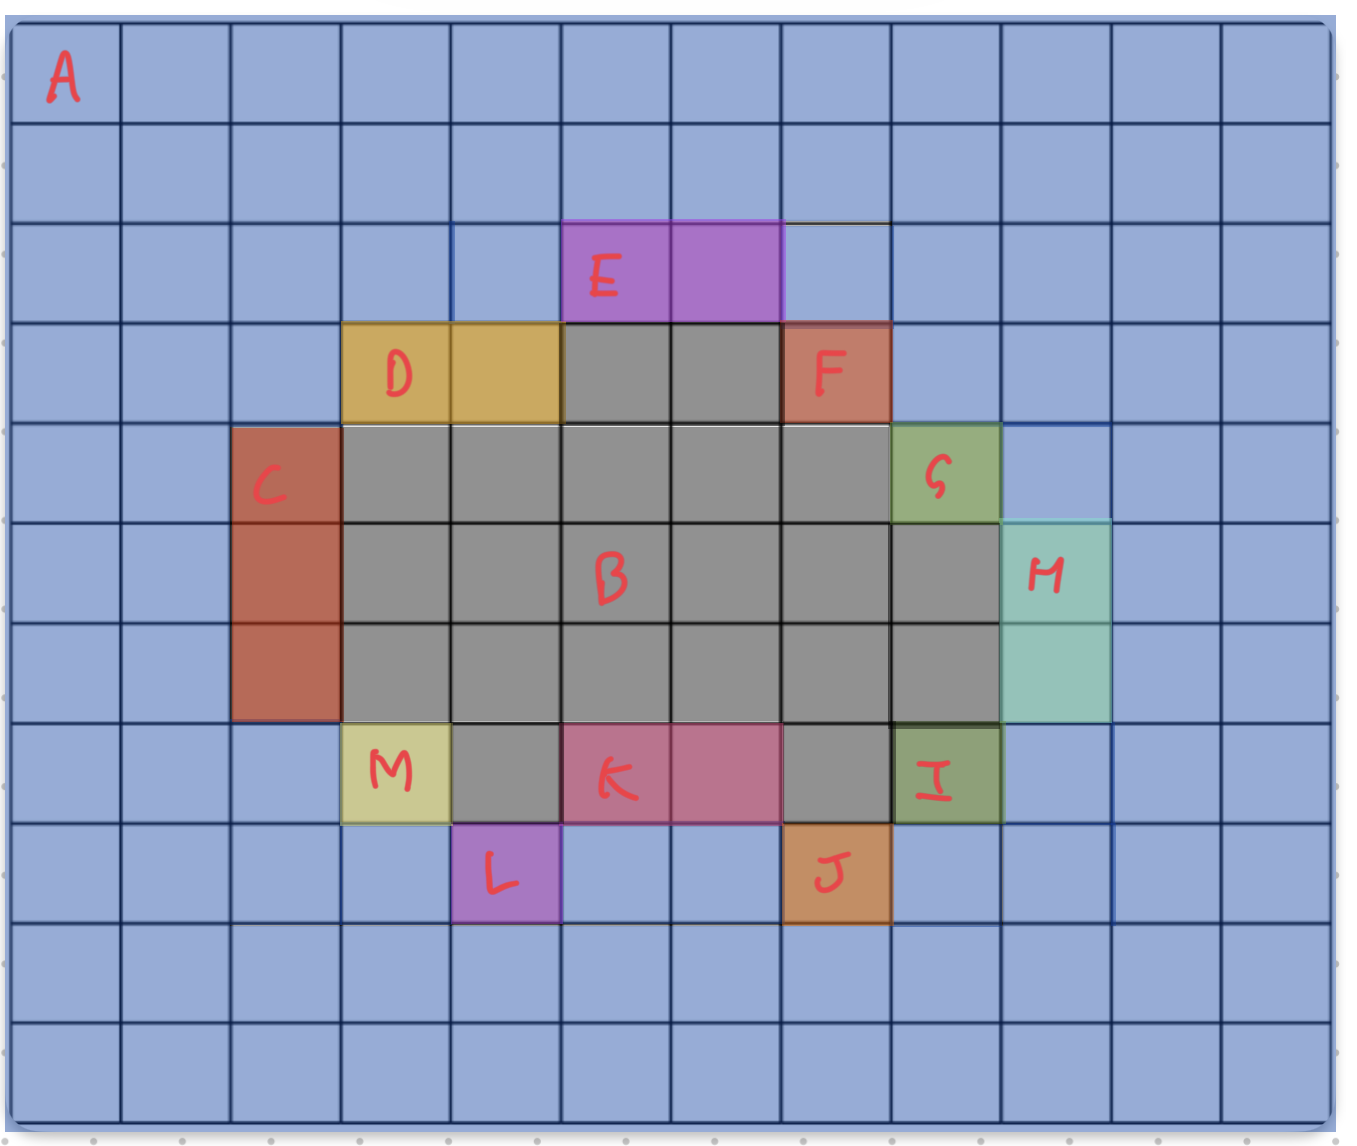
\includegraphics[width=0.6\linewidth]{figs/d4_connected_image.png}
    \caption{$d_4$ connectivity applied on the given image}
\end{figure}
%insert d4 connectivity example image
%insert d4 conenctivity colored image
\begin{itemize}
    \item There are a total of 13 4-connected structures
    \begin{itemize}
        \item Two white structures (interior and the exterior)
        \item Eleven gray structures
    \end{itemize}
\end{itemize}

From Figure %%%%ref figure and backspace
we can see that the longest gray structure has an area of 3 pixels

This approach does not follow Jordan's curve theorem as 4-connectivity of the pixels does not make a simple closed curve.

\subsection{Applying d8 connectivity}

d8 connectivity is defined as the connectivity of a pixel to the neighbors on its vertical, horizontal and diagonal axes (Akin to a queen in chess). \newline
\begin{figure}[h]
    \centering
    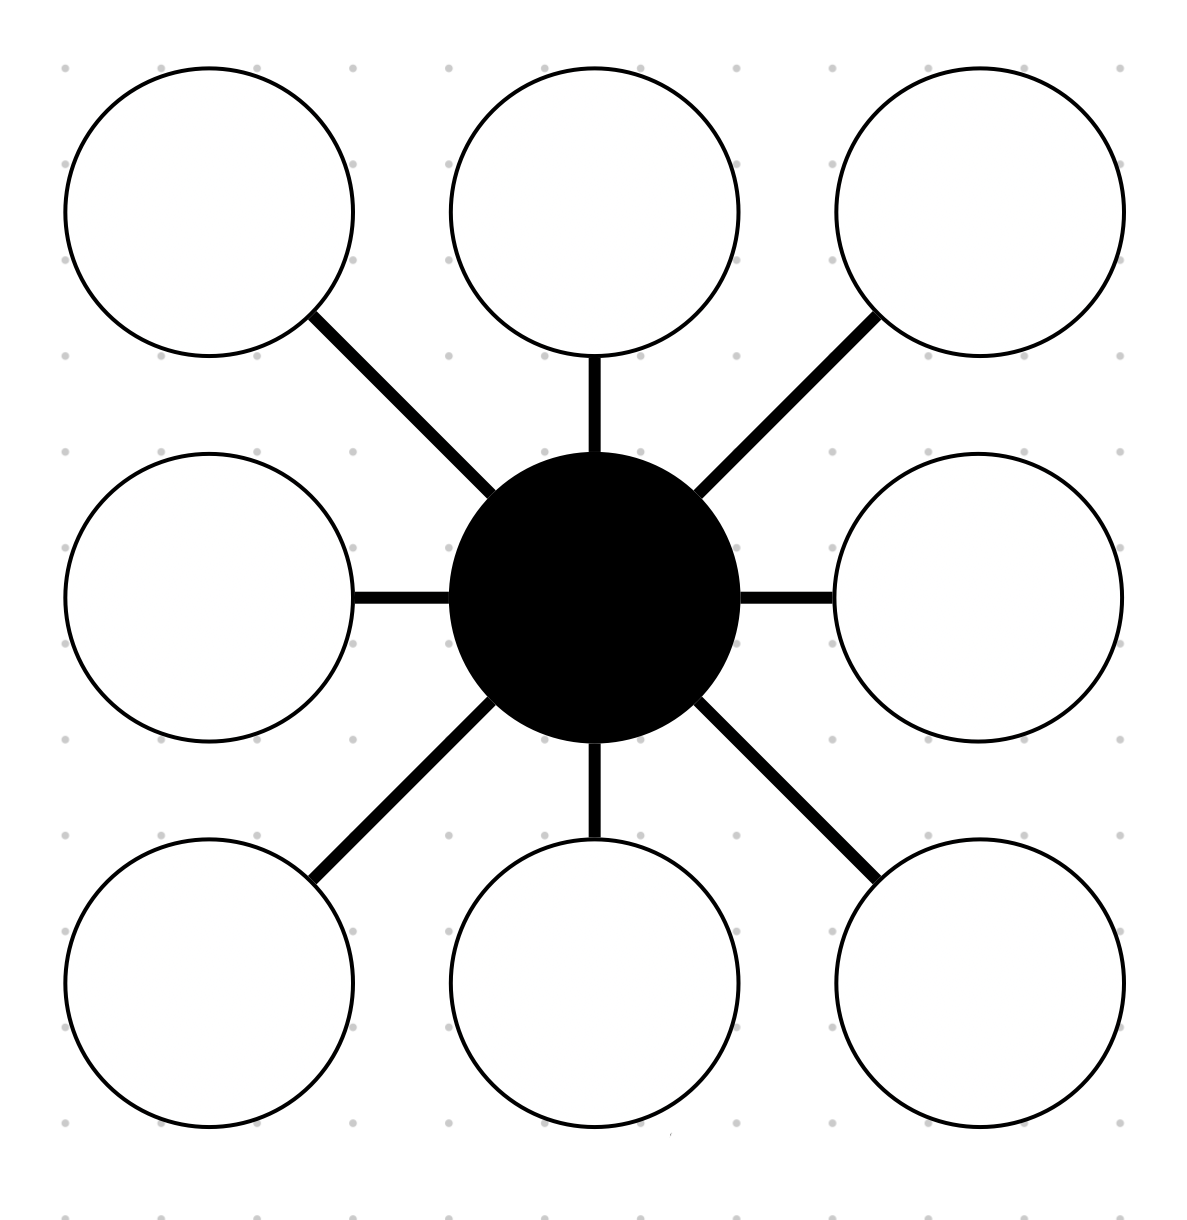
\includegraphics[width=0.4\linewidth]{figs/d8_connectivity.png}
    \caption{An example of $d_8$ connectivity}
\end{figure}
\newline
On computing the d8 connectivity of the given image, we get the following regions
\begin{figure}[h]
    \centering
    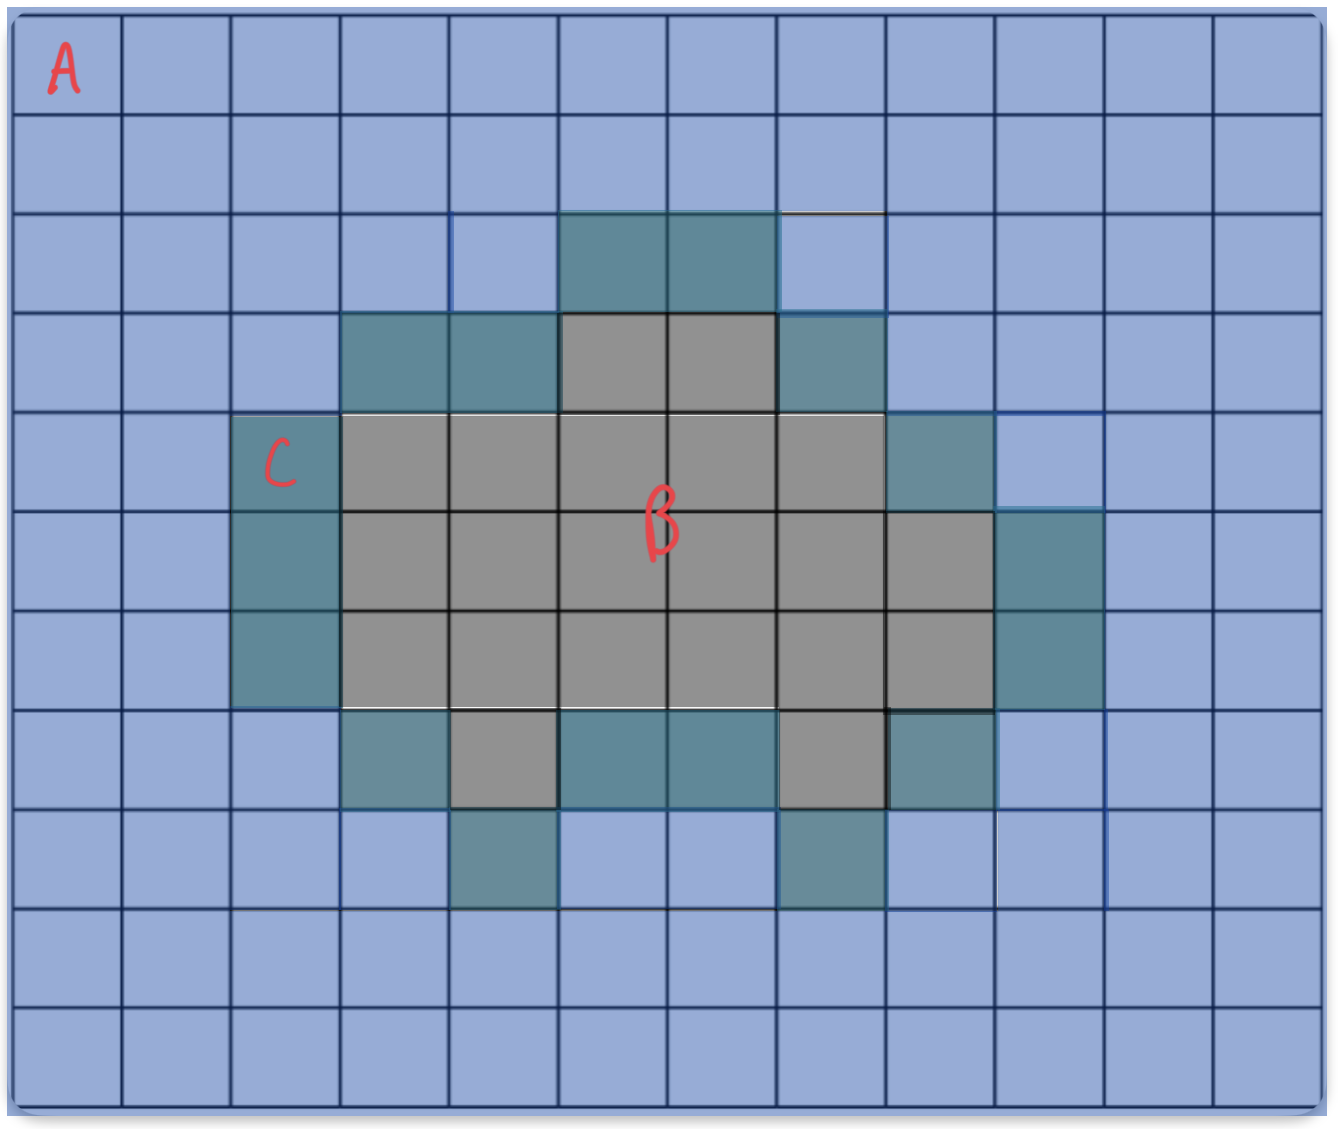
\includegraphics[width=0.6\linewidth]{figs/d8_connected_image.png}
    \caption{$d_8$ connectivity applied on the given image}
\end{figure}

%insert d8 conenctivity colored image
\begin{itemize}
    \item There are a total of 3 8-connected structures
    \begin{itemize}
        \item Two white structures (interior and the exterior)
        \item One gray structure (curve)
    \end{itemize}
\end{itemize}

From Figure %%%%ref figure and backspace
we can see that the longest gray structure has an area of 17 pixels. \newline

Yes, this approach does follow Jordan's curve theorem as d8 connectivity can make the gray pixels into a simple closed curve, dividing the area of the image into an interior and an exterior.



\subsection{Applying 6-C connectivity}

6-C connectivity is defined as the connectivity of a pixel to the neighbors on its vertical, horizontal and \textbf{only one} diagonal axes.
\newline
\begin{figure}[H]
    \centering
    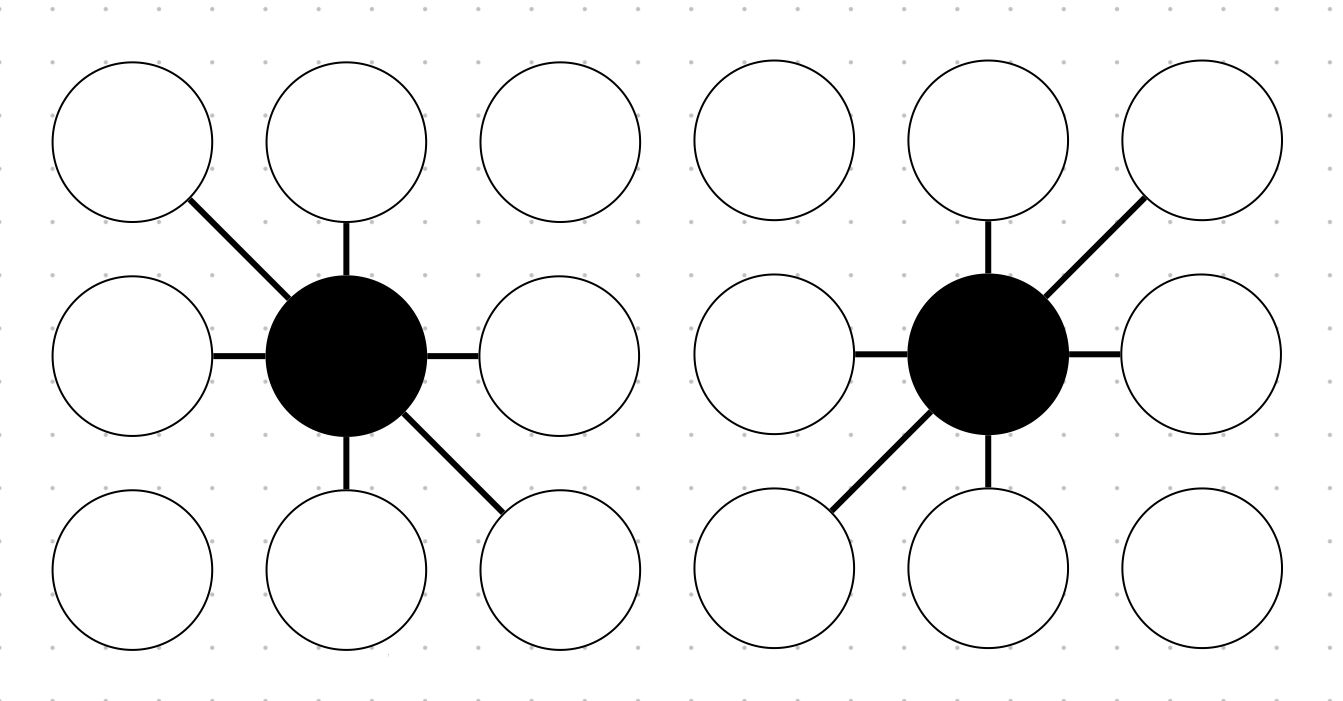
\includegraphics[width=0.6\linewidth]{figs/6c_connectivity.png}
    \caption{Examples of 6-$c$ connectivity}
\end{figure}
On computing the 6-C connectivity of the given image, we get the following regions
\begin{figure}[h]
    \centering
    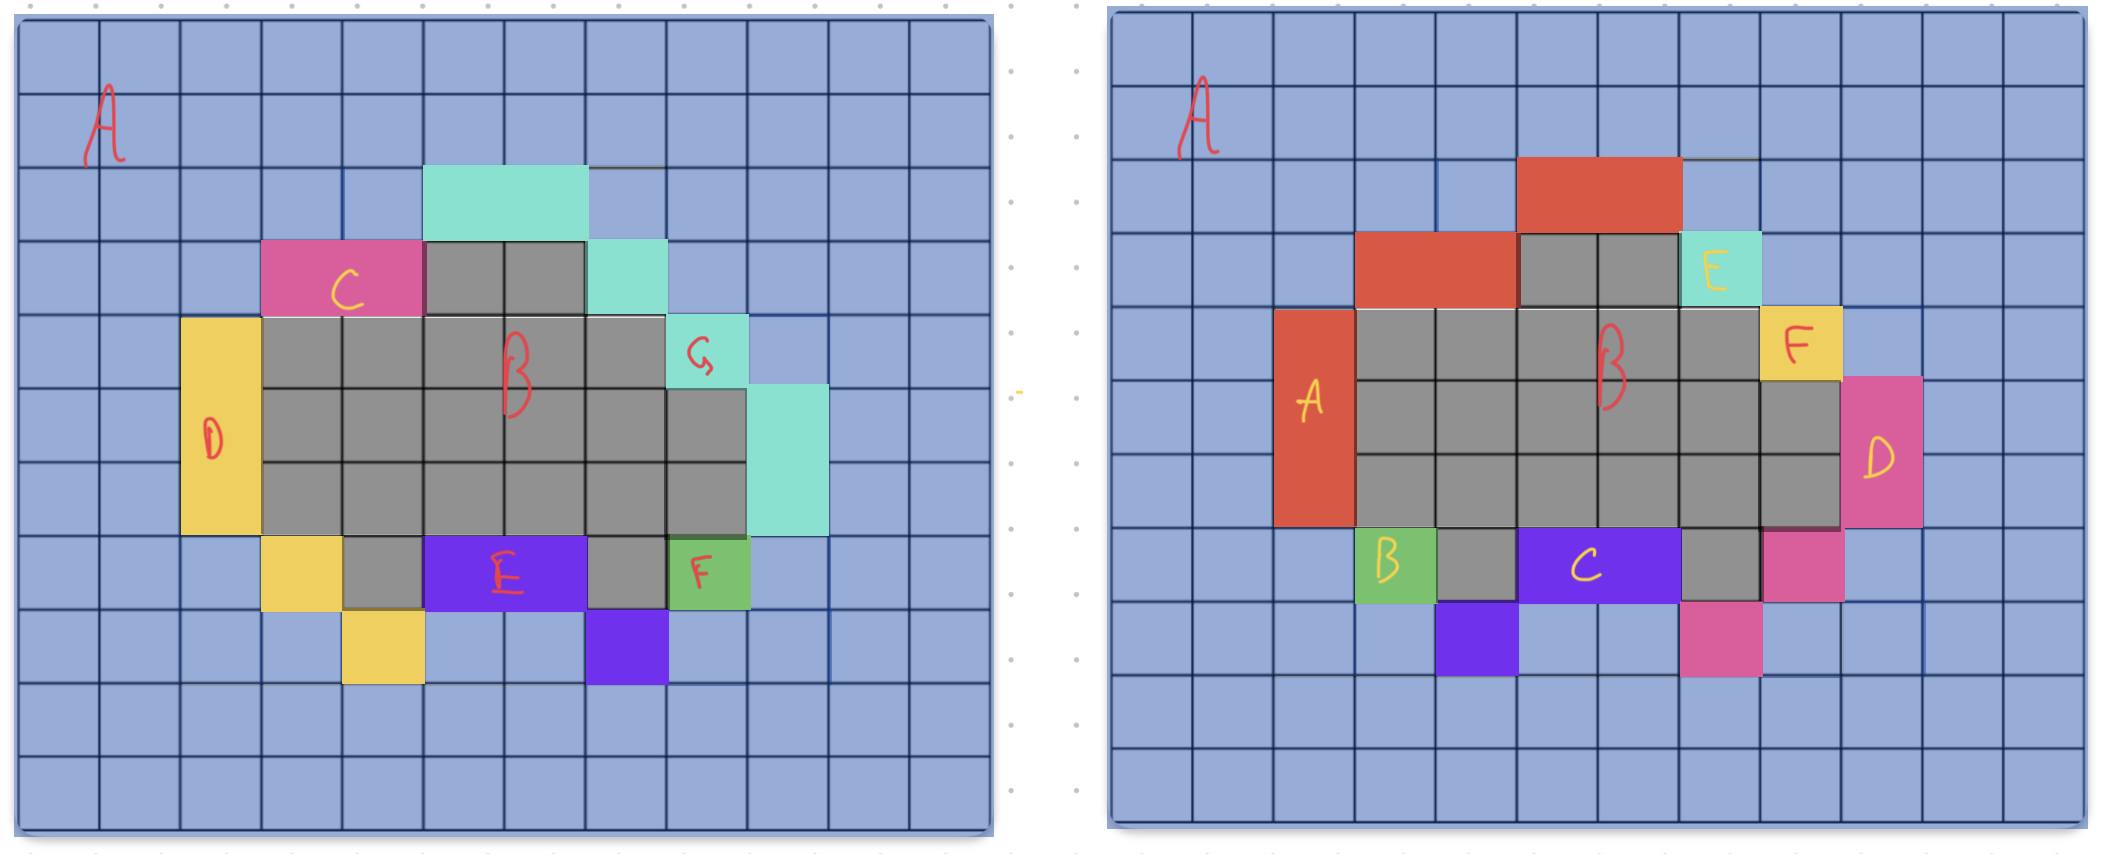
\includegraphics[width=0.8\linewidth]{figs/6c_connected_image.png}
    \caption{6C Connectivity applied on the given image}
\end{figure}
\begin{itemize}
    \item On using the first definition of 6-C connectivity, we get a total of 7 structures
    \begin{itemize}
        \item Two white structures (interior and the exterior)
        \item Five gray structures
    \end{itemize}
    \item On using the alternative definition of 6-C connectivity, we get a total of 7 structures
    \begin{itemize}
        \item Two white structures (interior and exterior)
        \item Six gray structures
    \end{itemize}
\end{itemize}
\newline
From Figure %%%%ref figure and backspace
we can see that the longest gray structure has an area of 6 pixels in the first case and 7 pixels in the second case.
\newline
This approach will not follow Jordan's curve theorem in either case as 6-C connectedness of the pixels does not make a simple closed curve in either case.





\section{1 Dimensional Filters}
\subsection{Box Filter Application}

The box filter of size 3 on a signal can be defined as:
$${y[i] = \frac{1}{3} \large\sum _{k=-1}^{1} x[i+k]}$$
\newline
where $y[i]$ is the transformed signal at time $i$ and $x[i]$ is the input signal at time $i$.
\newline
Using this formula, we get:\newline

${y[1] = \frac{1}{3} \large\sum _{k=-1}^{1} x[1+k] = \frac{1}{3} (0+1+1) = \frac{2}{3} \Rightarrow y[1]=  0.67 }$\newline

${ y[2] = \frac{1}{3} \large\sum _{k=-1}^{1} x[2+k] = \frac{1}{3} (1+1+1) = \frac{3}{3} \Rightarrow y[2]=  1 }$ \newline

${ y[3] = \frac{1}{3} \large\sum _{k=-1}^{1} x[3+k] = \frac{1}{3} (1+1+5) = \frac{7}{3} \Rightarrow y[3]=  2.34 }$ \newline

${ y[4] = \frac{1}{3} \large\sum _{k=-1}^{1} x[4+k] = \frac{1}{3} (1+5+1) = \frac{7}{3} \Rightarrow y[4]=  2.34 }$ \newline

${ y[5] = \frac{1}{3} \large\sum _{k=-1}^{1} x[5+k] = \frac{1}{3} (5+1+1) = \frac{7}{3} \Rightarrow y[5]=  2.34 }$ \newline

${ y[6] = \frac{1}{3} \large\sum _{k=-1}^{1} x[6+k] = \frac{1}{3} (1+1+1) = \frac{3}{3} \Rightarrow y[6]=  1 }$ \newline

${ y[7] = \frac{1}{3} \large\sum _{k=-1}^{1} x[7+k] = \frac{1}{3} (1+1+5) = \frac{7}{3} \Rightarrow y[7]=  2.34 }$ \newline

${ y[8] = \frac{1}{3} \large\sum _{k=-1}^{1} x[8+k] = \frac{1}{3} (1+5+5) = \frac{11}{3} \Rightarrow y[8]=  3.67 }$ \newline

${ y[9] = \frac{1}{3} \large\sum _{k=-1}^{1} x[9+k] = \frac{1}{3} (5+5+5) = \frac{15}{3} \Rightarrow y[9]=  5 }$ \newline

${ y[10] = \frac{1}{3} \large\sum _{k=-1}^{1} x[10+k] = \frac{1}{3} (5+5+5) = \frac{15}{3} \Rightarrow y[10]=  5 }$ \newline

${ y[11] = \frac{1}{3} \large\sum _{k=-1}^{1} x[11+k] = \frac{1}{3} (5+5+5) = \frac{15}{3} \Rightarrow y[11]=  5 }$ \newline

${ y[12] = \frac{1}{3} \large\sum _{k=-1}^{1} x[12+k] = \frac{1}{3} (5+5+4) = \frac{14}{3} \Rightarrow y[12]=  4.67 }$ \newline

${ y[13] = \frac{1}{3} \large\sum _{k=-1}^{1} x[13+k] = \frac{1}{3} (5+4+3) = \frac{12}{3} \Rightarrow y[13]=  4 }$ \newline

${ y[14] = \frac{1}{3} \large\sum _{k=-1}^{1} x[14+k] = \frac{1}{3} (4+3+2) = \frac{9}{3} \Rightarrow y[14]=  3 }$ \newline

${ y[15] = \frac{1}{3} \large\sum _{k=-1}^{1} x[15+k] = \frac{1}{3} (3+2+1) = \frac{6}{3} \Rightarrow y[15]=  2 }$ \newline

${ y[16] = \frac{1}{3} \large\sum _{k=-1}^{1} x[16+k] = \frac{1}{3} (2+1+1) = \frac{4}{3} \Rightarrow y[16]=  1.34 }$ \newline

${ y[17] = \frac{1}{3} \large\sum _{k=-1}^{1} x[17+k] = \frac{1}{3} (1+1+0) = \frac{2}{3} \Rightarrow y[17]=  0.67 }$ \newline

Therefore, the attenuated signal becomes: \newline
\begin{center}
\begin{tabular}{|c|c|c|c|c|c|c|c|c|c|c|c|c|c|c|c|c|c|c|}
\hline
 0 \cellcolor{lightgray}&0.67&1&	2.34&	2.34&	2.34&	1&	2.34&	3.67&	5&	5&	5&	4.67&	4&	3&	2&	1.34&	0.67&	0 \cellcolor{lightgray}\\
 \hline
\end{tabular}
\end{center}

\subsection{Attenuation}

\begin{figure}[H]
    \centering
    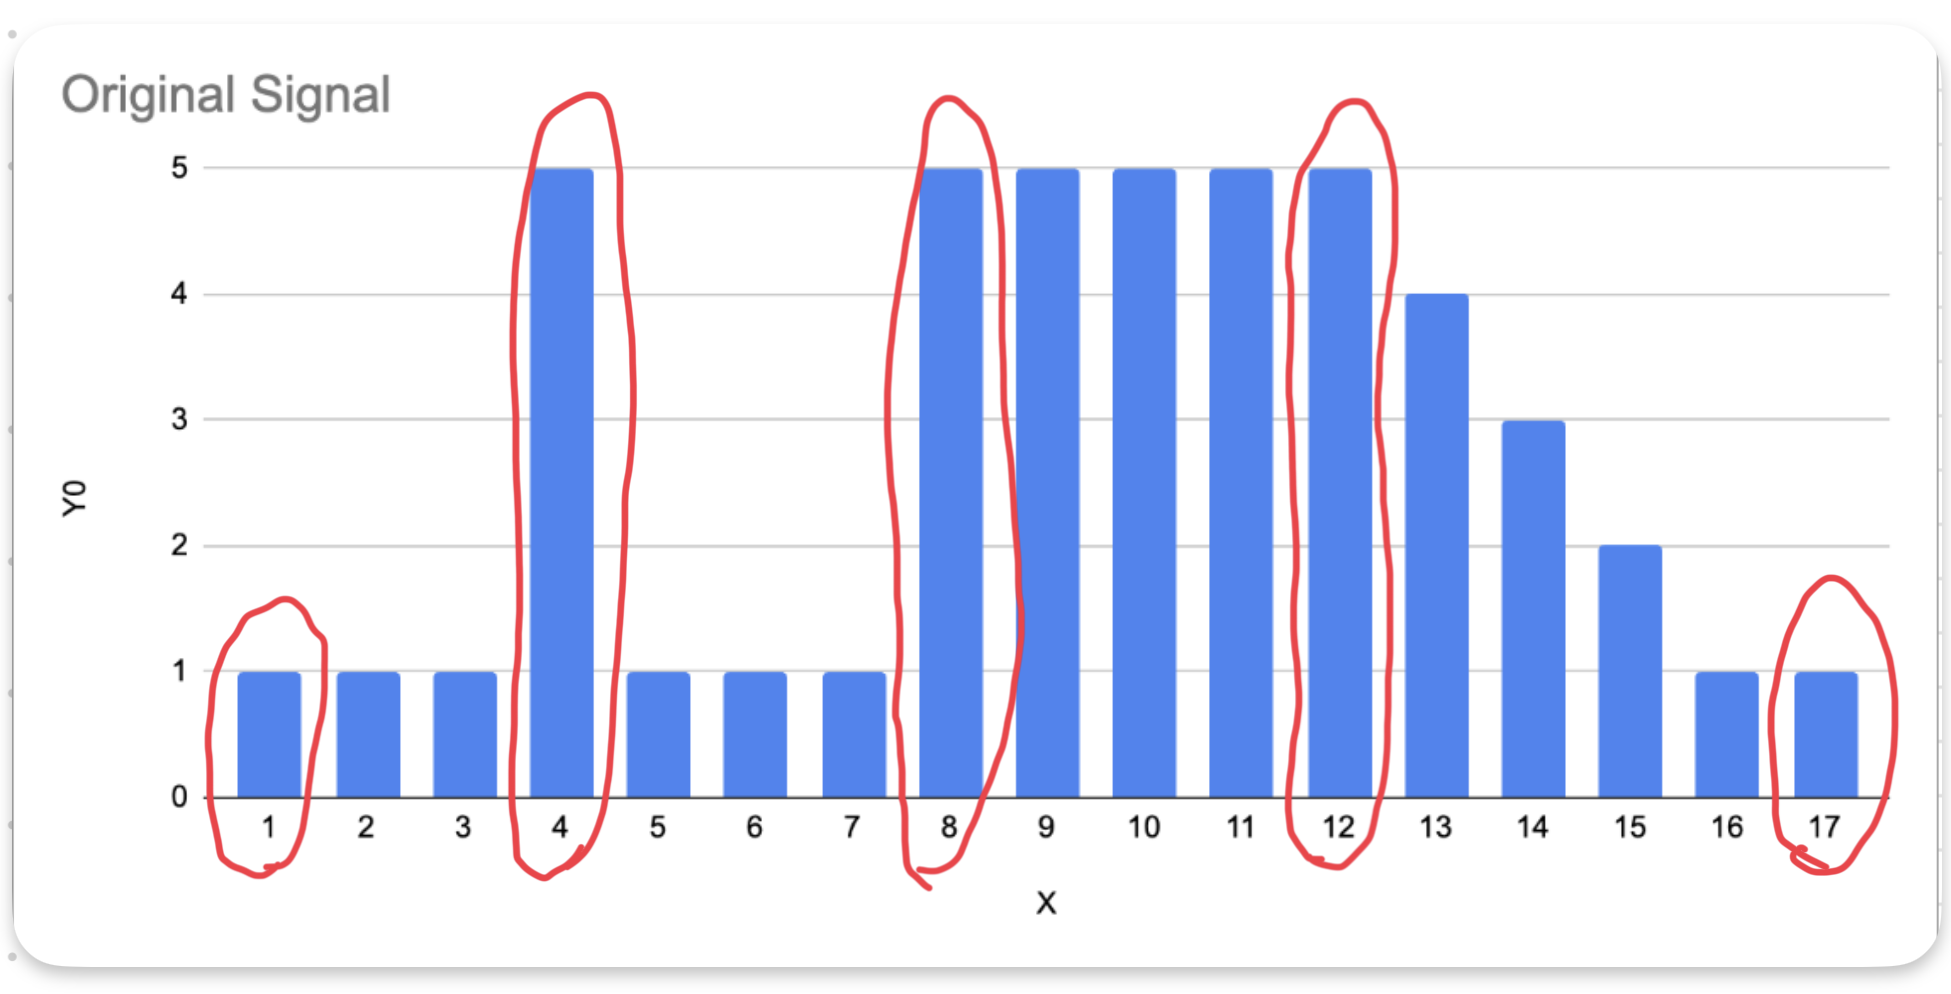
\includegraphics[width=0.5\linewidth]{figs/original_signal_graph.png}
    \caption{Original signal plotted with the attenuation in the signal encircled in red}
    \label{fig:og_signal}
\end{figure}
\begin{figure}[H]
    \centering
    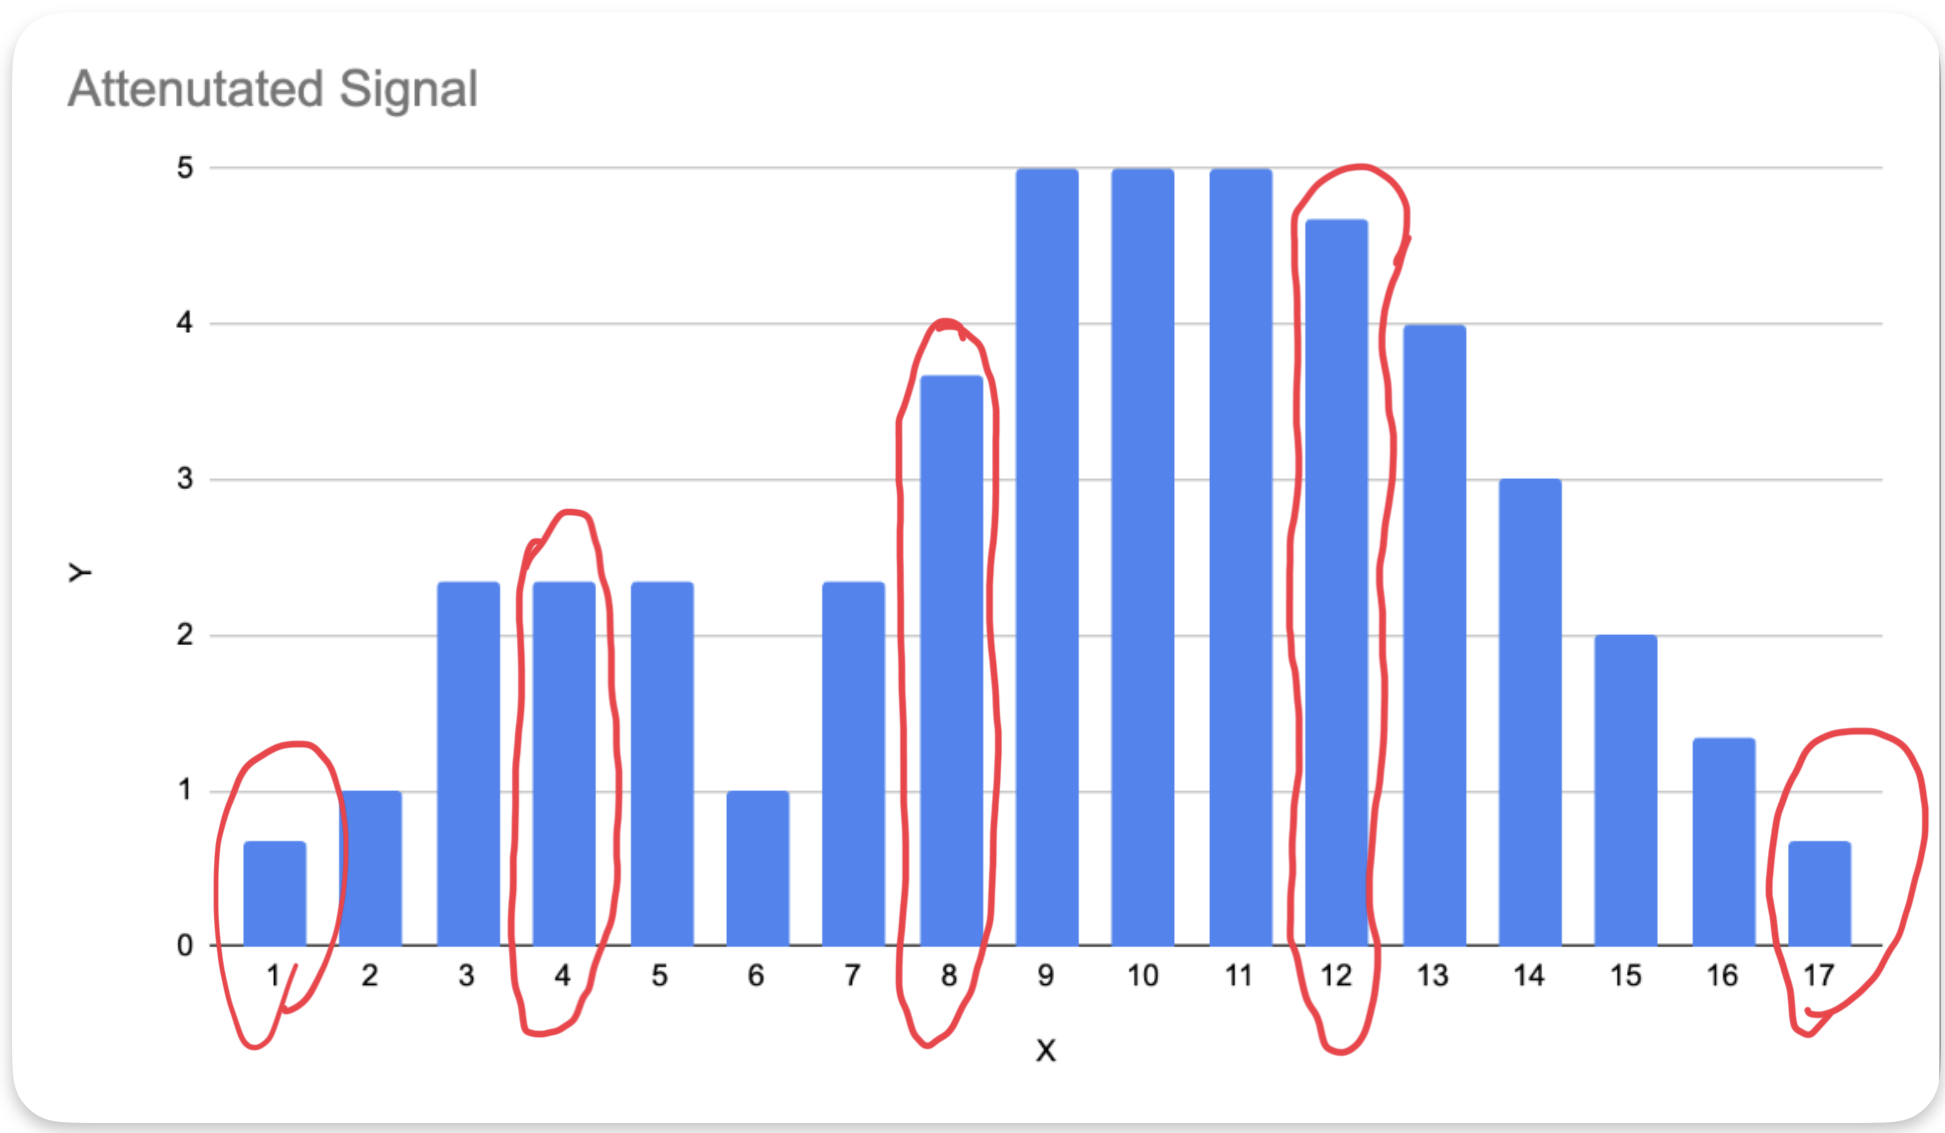
\includegraphics[width=0.5\linewidth]{figs/attenuated_signal_graph.png}
    \caption{(Transformed signal plotted with the attenuation in the signal encircled in red}
    \label{fig:att_signal}
\end{figure}


From Figures \ref{fig:og_signal} and \ref{fig:att_signal}, we can see that the signal has been attenuated at times $i= 1,4,8,12,17$
\subsubsection{At $i=1$ and $i=17$}
Due to zero-padding along the edges of the signal, the signal value of 1 at times $i=1$ and $i=17$ has been attenuated to $0.67$

\subsubsection{At $i=4$ and $i=8$}
The frequency of signal $x[i]$ suddenly jumps to 5 at $i=4$ and $i=8$. Due to the smoothening effect of the box filter, the filtered value of the signal gets attenuated.

\subsubsection{At $i=12$}
The frequency of the signal x[i] starts reducing at $i=12$ from $x[12]=5$ to $x[16]=1$, The box filter smoothens the frequency at $x[12]$ using the values around it ($x[11]$ and $x[13]$) attenuating the signal.


\subsection{Linearity of Box Filters}

The box filter is defined as:

\begin{equation}
\large T(x)[n] = \frac{1}{2k+1} \sum_{i=-k}^{k} x[n+i] 
\end{equation}


Using this definition, putting $x=ax_1 + bx_2$ , the equation becomes:

\[
\large T(ax_1 + bx_2)[n] = \frac{1}{2k+1} \sum_{i=-k}^{k} (ax_1+bx_2)[n+i]
\]
\[
\Rightarrow \large T(ax_1 + bx_2)[n] = \frac{1}{2k+1} \sum_{i=-k}^{k}(ax_1[n+i]  +bx_2[n+i])
\]
\[
\Rightarrow \large T(ax_1 + bx_2)[n] = \frac{1}{2k+1} ( \sum_{i=-k}^{k}ax_1[n+i]  + \sum_{i=-k}^{k}bx_2[n+i])
\]
\[
\Rightarrow \large T(ax_1 + bx_2)[n] = \frac{1}{2k+1} ( \sum_{i=-k}^{k}ax_1[n+i]  + \sum_{i=-k}^{k}bx_2[n+i])
\]
\[
\Rightarrow \large T(ax_1 + bx_2)[n] = \frac{1}{2k+1} \sum_{i=-k}^{k}ax_1[n+i]  + \frac{1}{2k+1}\sum_{i=-k}^{k}bx_2[n+i]
\]
\[
\Rightarrow \large T(ax_1 + bx_2)[n] = \frac{1}{2k+1}a \sum_{i=-k}^{k}x_1[n+i]  + \frac{1}{2k+1}b\sum_{i=-k}^{k} x_2[n+i]
\]

\[
\Rightarrow \large T(ax_1 + bx_2)[n] = \large aT(x_1)[n] +bT(x_2)[n]
\]
\newline
Hence, we can say that the average box filter is indeed a \textbf{linear filter.}
\subsection{Shift Invariance of global mean subtraction filter}

A filter ${y[t] = T(x[t])}$ on signal $x[t]$ is defined as Shift Invariant if ${y[t-\tau] =T(x[t-\tau])}$ where $\tau$ is a temporal shift (change in time).
\newline
\newline We define a transformation ${y[t] = V(x[t])}$ where ${V(x[t]) = x[t] - \mu}$ , where $\mu$ is defined as the global average mean of the signal. (${\mu = \int_{0}^{T} x[t] dt}$).
\newline
\newline For a finite signal the value of $\mu$ will be constant. 
\newline
\newline To show that ${y[t-\tau] =V(x[t-\tau])}$ :
\newline
\newline Solving LHS: 
\[
y[t] = x[t]- \mu
\]
\begin{center}
For $t = t-\tau$ (Shifting the transformed signal by $\tau$)
\end{center}
\begin{equation}
\label{one}
    y[t-\tau] = x[t-\tau] - \mu
\end{equation}
\newline
Solving RHS:
\[
V(x[t]) = x[t]- \mu
\]
\begin{center}
For $t = t-\tau$ (Transforming the shifted signal)
\end{center}
\begin{equation}
\label{two}
    V([t-\tau]) = x[t-\tau] - \mu
\end{equation}
\newline
From Equations \ref{one} and \ref{two} we can say that ${y[t-\tau] =V(x[t-\tau])}$ , which proves the linearity of the given filter ${V(x[t]) = x[t] - \mu}$ .


\subsection{Linearity of Median filter}

A convolution is defined as a linear filter which is shift invariant (\ref{book}). A linear filter $g(I)$ is a filter which satisfies the property $$g(\alpha I_1 + \beta I_2) = \alpha g(I_1) + \beta g(I_2)$$
\newline
To prove the median filter is not a linear filter, we assume a median filter of box size 5, two constants $\alpha = 3$ and $\beta = 2$ , and two 1D signals as follows
$$I_1 = [1,4,6,10,13]$$
$$I_2 = [7,3,21,47,23]$$
\newline
Computing $g(\alpha I_1 + \beta I_2)$ :

\[ 
    g(\alpha I_1 + \beta I_2) = g( 3*[1,4,6,10,13] + 2*[7,3,21,47,23])
\]
\[ 
    g(\alpha I_1 + \beta I_2) = g([3,12,18,30,39] + [14,6,42,94,46])
\]
\[ 
    g(\alpha I_1 + \beta I_2) = g([17,18,60,124,85])
\]
\begin{equation}
\label{median_LHS}
    g(\alpha I_1 + \beta I_2) = 60
\end{equation}
\newline
Computing $ \alpha g(I_1) + \beta g(I_2)$ :

\[
\alpha g(I_1) + \beta g(I_2) = 3 * g([1,4,6,10,13]) + 2*g([14,6,42,94,46])
\]
\[
\alpha g(I_1) + \beta g(I_2) = 3 * 6 + 2*g([14,6,42,94,46])
\]
\[
\alpha g(I_1) + \beta g(I_2) = 3 * 6 + 2*42
\]
\[
\alpha g(I_1) + \beta g(I_2) = 18 + 84
\]
\begin{equation}
\label{median_RHS}
\Rightarrow \alpha g(I_1) + \beta g(I_2) = 102
\end{equation}
\newline
From equations \ref{median_LHS} and \ref{median_RHS}, we can see that $60 \ne 102$ , which violates the linearity property.
\newline
$\therefore$ The median filter cannot be called convolution, as it violates the property of linearity.

\section{2D Filters and Fourier Transforms}
\subsection{Sobel Filter Complexity}
A vertical edge sobel filter can be defined as follows:
\[
\frac{1}{8}
\begin{bmatrix}
     -1&-2&-1\\
     0&0&0\\
     1&2&1
\end{bmatrix}
\]
\newline
Its decomposition can be defined as follows:
\[
\frac{1}{2}
\begin{bmatrix}
    1\\0\\-1
\end{bmatrix}
\begin{bmatrix}
    1&2&1
\end{bmatrix}
\]
\newline
Assuming a $n \times n$ image with zero padding (making the size of the image $n+2 \times n+2$, $\alpha$ as a constant computation cost of non-zero multiplications, and $\beta$ as the constant computation cost of non-zero addition, the number of operations required to apply the non-decomposed filter to the entire image will be as following (Assuming multiplication by 0,1 and -1 as taking no effective computation time)
\newline
Assuming a following pixel
\[
\begin{bmatrix}
     a&b&c\\
     d&e&f\\
     g&h&i
\end{bmatrix}
\]
\newline
The Convolution becomes:
\[
\begin{bmatrix}
     a&b&c\\
     d&e&f\\
     g&h&i
\end{bmatrix}
 \otimes \frac{1}{8}\begin{bmatrix}
     -1&-2&-1\\
     0&0&0\\
     1&2&1
\end{bmatrix}
\]

\[
\Rightarrow \frac{1}{8}\begin{bmatrix}
     -1.a+-2.b+-1.c\\
     0.d+0.e+0.f\\
     1.g+2.h+1.i
\end{bmatrix}
\]

\[
\Rightarrow \frac{1}{8}\begin{bmatrix}
     -1.a+-2.b+-1.c\\
     0.d+0.e+0.f\\
     1.g+2.h+1.i
\end{bmatrix}
\]
\[
\Rightarrow \frac{1}{8}\begin{bmatrix}
     -a+-2b+-c+0+g+2h+i
\end{bmatrix}
\]
\newline
This operation takes 3 multiplication (multiplication by 2 and normalization) steps and 4 addition steps per pixel. Therefore, for $n+2 \times n+2$ pixels, the computation time defined as 
\begin{equation}
\label{composed}
C_{non\_seperable} = (3 \alpha+4\beta)n^2
\end{equation}
\newline
Now, for the linearly decomposed filter, passing the same pixel through the filter and calculating the computation cost.

\[
\begin{bmatrix}
     a&b&c\\
     d&e&f\\
     g&h&i
\end{bmatrix}
 \otimes \begin{bmatrix}
     1&\\
     0\\
     -1
\end{bmatrix}
\]
\[
\Rightarrow \begin{bmatrix}
    a.1+0.d-1.g & b.1+0.e-1.h & c.1+0.f-1.i
\end{bmatrix}
\]
\[
\Rightarrow \begin{bmatrix}
    a-g & b-h & c-i
\end{bmatrix}
\]
\[
\Rightarrow \begin{bmatrix}
    a-g & b-h & c-i
\end{bmatrix} \otimes \begin{bmatrix}
    1&2&1
\end{bmatrix} \times\frac{1}{2}
\]
\[
\Rightarrow \frac{1}{2} \begin{bmatrix}
    a-g+2b-2h+c+i
\end{bmatrix}
\]
\newline
This operation takes 3 multiplication steps (multiplication by 2 and normalization) and 8 addition steps per pixel. Therefore, for $n+2 \times n+2$ pixels, the computation cost for a linearly separable filter is defined as 
\begin{equation}
\label{seperable}
    C_{separable} = (2 \alpha + 8 \beta) n^2
\end{equation}

For the usage of linearly separable filter, the inequality $C_{non\_seperable} > C_{separable}$ must hold. From Equations \eqref{composed} and \eqref{seperable}:

\[
C_{non\_seperable} > C_{separable}
\]
\[
(3 \alpha+4\beta)n^2 > (2 \alpha + 8 \beta) n^2
\]
\[
(\alpha-4\beta)n^2>0
\]
\newline
As $\alpha - 4\beta$ is a constant, assuming it as $C$
\[
Cn^2>0
\]
\[
n^2>0
\]
\newline
As $n^2>0$ is true $\forall \space n \in \mathbb{N}$, we can say that it is feasible to use the linearly separable filter for any size of image. Therefore the minimum image size where the separable filter becomes feasible is $1 \times 1$.
\subsection{Fast Fourier Transform}
The Discrete Fourier Transform for each point in a frequency domain $k,l$ is defined as
\[
\scalebox{1.5}{$F[k,l] = \frac{1}{MN} \sum_{m=0}^{M-1}\sum_{n=0}^{N-1} f[m,n]e^{-j2\pi(\frac{k}  {M}m + \frac{l}{N}n)}$} 
\]
\newline
\[
\scalebox{1.2}{$ \Rightarrow F[k,l] = \frac{1}{MN} \sum_{m=0}^{M-1} \sum_{n=0}^{N-1}f[m,n]e^{-2j\pi.m\frac{k}{M}}.e^{-2j\pi.n\frac{l}{N}} $} 
\]
\newline
\[
\scalebox{1.2}{$
\Rightarrow F[k,l] = \frac{1}{M}\sum_{m=0}^{M-1}(\frac{1}{N}\sum_{n=0}^{N-1}f[m,n]\ e^{-2j\pi.n\frac{l}{N}})\ e^{-2j\pi.m\frac{k}{M}}
$}
\]
\newline
The term:
\[
\frac{1}{N}\sum_{n=0}^{N-1}f[m,n]\ e^{-2j\pi.n\frac{l}{N}}
\]
\newline
in the above equation is defined as a Discrete Fourier Transform in one dimension. The Fast Fourier Transform algorithm of a 1-dimensional signal is defined as:
\begin{algorithm}
\caption{1D Fast Fourier Transform}\label{fft}
\begin{algorithmic}[1]
\Function{FFT}{$[a_0,...a_N-1,\omega,N$}
\If{$N=0$} \Return{$[a_0]$} \EndIf
\State $F_{\text{even}} \gets \text{FFT}([a_0, a_2,..., a_{N-2}], \omega^2, N/2)$
    \State $F_{\text{odd}} \gets \text{FFT}([a_1, a_3,..., a_{N-1}], \omega^2, N/2)$
    \State $F \gets$ new vector of length $N$
    \State $x \gets 1$
    \For{$j = 0$ to $N-1$}
        \State $F[j] \gets F_{\text{even}}[j \bmod (N/2)] + x.F_{\text{odd}}[j \bmod (N/2)]$
        \State $x \gets x \cdot \omega$
    \EndFor
    \State \Return $F$
\EndFunction
\end{algorithmic}
\end{algorithm}

From Algorithm \eqref{fft}, we can say that the FFT Algorithm calls itself recursively on half the input size ($N/2$) and performs $N$ operations in combining the result. 
\newline
The Master Theorem is  a formula which can be used to define the runtime of recursive algorithms, and is defined as:
\newline
\begin{equation}
\label{mastertheorem}
    \scalebox{1.15}{$T(n) = aT(\frac{n}{b}) + g(n) \ \forall\  a \geq 1,\  b > 1$}
\end{equation}
From algorithm \ref{fft} and equation \eqref{mastertheorem}, we can say that the Fast Fourier Transform can be represented in the form of the master theorem when $a=2$ (two sub problems) and $b=2$ (each subproblem is a size of $n/2$). Since the for-loop in FFT takes $O(n)$ time, the asymptotic bound of $T(n)$ becomes
\[
g(n) = \Theta(n^{\log_ba)}
\]
\[
g(n) = \Theta(n^{\log_22)}
\]
\newline
In this case, the value of $T(n)$ becomes $\Theta(n^{\log_ba}\log n)$. And (since $log_22 = 1$), we can say that the run time of a one-dimensional Fourier transform is $\Theta(n\log n)$ 

Since a two-dimensional fourier transform is a one dimensional fourier transform transformed in the frequency range of the other dimension's signal. Hence we defined the inner transform with the frequency range of $N$ and the outer transform with the frequency range of $M$, the overall run time is multiplied by a factor of $M$.
\newline
Therefore the final runtime of applying a Fast Fourier Transform to a two dimensional signal becomes:
\begin{equation}
    \Theta(MN\log N)
\end{equation}
\section{References}
\nocite{*}
\printbibliography[heading=none]
%%%%%%%%%%%%%%%%%%%%%%%%%%%%%%%%%%%%%%%%%%%%%%%%%%%%%%%%%%%%

\end{document}